\section{Dexterous Hand Design / Optimization}
  \label{secHandDesign}

\newcommand{\bA}{\mathbf{A}}
\newcommand{\bB}{\mathbf{B}}
\newcommand{\bC}{\mathbf{C}}
\newcommand{\bD}{\mathbf{D}}
\newcommand{\bE}{\mathbf{E}}
\newcommand{\bF}{\mathbf{F}}
\newcommand{\bG}{\mathbf{G}}
\newcommand{\bH}{\mathbf{H}}
\newcommand{\bI}{\mathbf{I}}
\newcommand{\bJ}{\mathbf{J}}
\newcommand{\bK}{\mathbf{K}}
\newcommand{\bM}{\mathbf{M}}
\newcommand{\bR}{\mathbf{R}}
\newcommand{\bU}{\mathbf{U}}
\newcommand{\ba}{\mathbf{a}}
\newcommand{\bb}{\mathbf{b}}
\newcommand{\bc}{\mathbf{c}}
\newcommand{\bd}{\mathbf{d}}
\newcommand{\be}{\mathbf{e}}
\newcommand{\bff}{\mathbf{f}}
\newcommand{\bg}{\mathbf{g}}
\newcommand{\bk}{\mathbf{k}}
\newcommand{\bm}{\mathbf{m}}
\newcommand{\bn}{\mathbf{n}}
\newcommand{\bp}{\mathbf{p}}
\newcommand{\bs}{\mathbf{s}}
\newcommand{\bt}{\mathbf{t}}
\newcommand{\bu}{\mathbf{u}}
\newcommand{\bv}{\mathbf{v}}
\newcommand{\bx}{\mathbf{x}}
\newcommand{\bl}{\mathbf{l}}
\newcommand{\bq}{\mathbf{q}}
\newcommand{\bw}{\vec{w}}
\newcommand{\bX}{\mathbf{X}}
\newcommand{\bS}{\mathbf{S}}
\newcommand{\bj}{\mathbf{j}}
\newcommand{\bT}{\mathbf{T}}
\newcommand{\bP}{\mathbf{P}}

\newcommand{\bbx}{\bar{\bx}}

%relevant work to discuss: http://biorobotics.harvard.edu/robotic_hand_optimization.html
%http://bbdl.usc.edu/Papers/2013_IJRR_Inouye_Anthropomorphic_Hand.pdf

Recent work has shown that carefully engineered mechanical designs can prove crucial in improving the versatility of robotic manipulators for static grasping tasks~\cite{Ciocarlie:2014:VGV:2674203.2674213}. The aim of our work is to generalize this concept in order to revolutionize dexterous manipulation in the same way. We therefore propose mathematical models and algorithmic approaches to co-design mechanical structures and control policies for robotic manipulation tasks. Our hypothesis is that by complementing each other and working in unison, control policies can be significantly simpler, and appropriate mechanical features -- joint stops, compliance, etc. -- can passively improve the robustness of the manipulation tasks while reducing sensing and actuation requirements. 

\subsection{Bottom-up design}

The design process will begin with a specific family of tasks (i.e., a Grasp Net). As described in Section~\ref{secLimitAnalysis}, features such as compliance of passive structures or joint limits can be computed through numerical optimization. Our goal is to automatically translate these optimized features into mechanical structures that can be 3D printed. As a first step, we will investigate bottom-up approaches. For the physical prototype of the 1 degree-of-freedom manipulator shown in Figure~\ref{SimpleExampleResults}, for example, we used a script to generate 3d printable geometry using constructive solid modeling. After fabrication, we used rubber bands to approximately match the optimized compliance of the passive features. The resulting mechanical setup was actuated manually. We view this first result as very encouraging because, with no sensing and very crude actuation, the simple robotic hand was able to reliably and repeatedly perform the manipulation task it was designed for.

Our future investigations will formalize the process we used to design and fabricate our first robotic
\begin{wrapfigure}{hR}{0.25\linewidth}
\vspace{-4mm}
\includegraphics[width=1.0\linewidth]{figs/bendy}
\vspace{-7mm}
\end{wrapfigure}hand. We will begin by building upon the mechanism design work led by PI Coros~\cite{Coros2013,Bacher2015} to automate the synthesis and optimization of assemblies based on trajectories of contact points. We will then extend these models to appropriately control the compliance of the mechanical structures. As illustrated in the inset figure, 3D printing is capable of fabricating objects with complex geometric features, which, in turn, allows the compliance of manufactured parts to be modulated. PI Coros has already started to develop computational methods to explore the relationship between geometric shape, material parameters and deformation behavior~\cite{Skouras2013,Jesus2015}. Briefly, we will model mechanical structures using a Finite Element Method (FEM) approach, where volumetric structures are discretized into a set of elementary shapes (e.g. tetrahedrons). Through a constitutive model, the deformations of the elementary shapes are mapped to elastic energy by integrating over the domain of each element. The global deformation energy $W$ is obtained by summing up elemental contributions, and internal forces are computed as $\textbf{f}_{int} = -\frac{\partial W}{\partial \bx}$, where $\bx$ is an array concatenating the vertex coordinates for each element. Quasi-static configurations for the mechanical structures under load can be obtained by finding the deformed configuration $\bx$ that leads to force equilibrium. Our mathematical models predict how these quasi-static configurations change with the shape of the mechanical parts and their material parameters~\cite{Skouras2013}. We will leverage these models to optimize the internal forces generated when mechanical parts deform as the robot hand performs manipulation tasks. To increase the range of materials that can be used, we will experiment with both 3D printing and laser cutting technologies to manufacture the mechanical components.

\begin{figure}
\begin{center}
{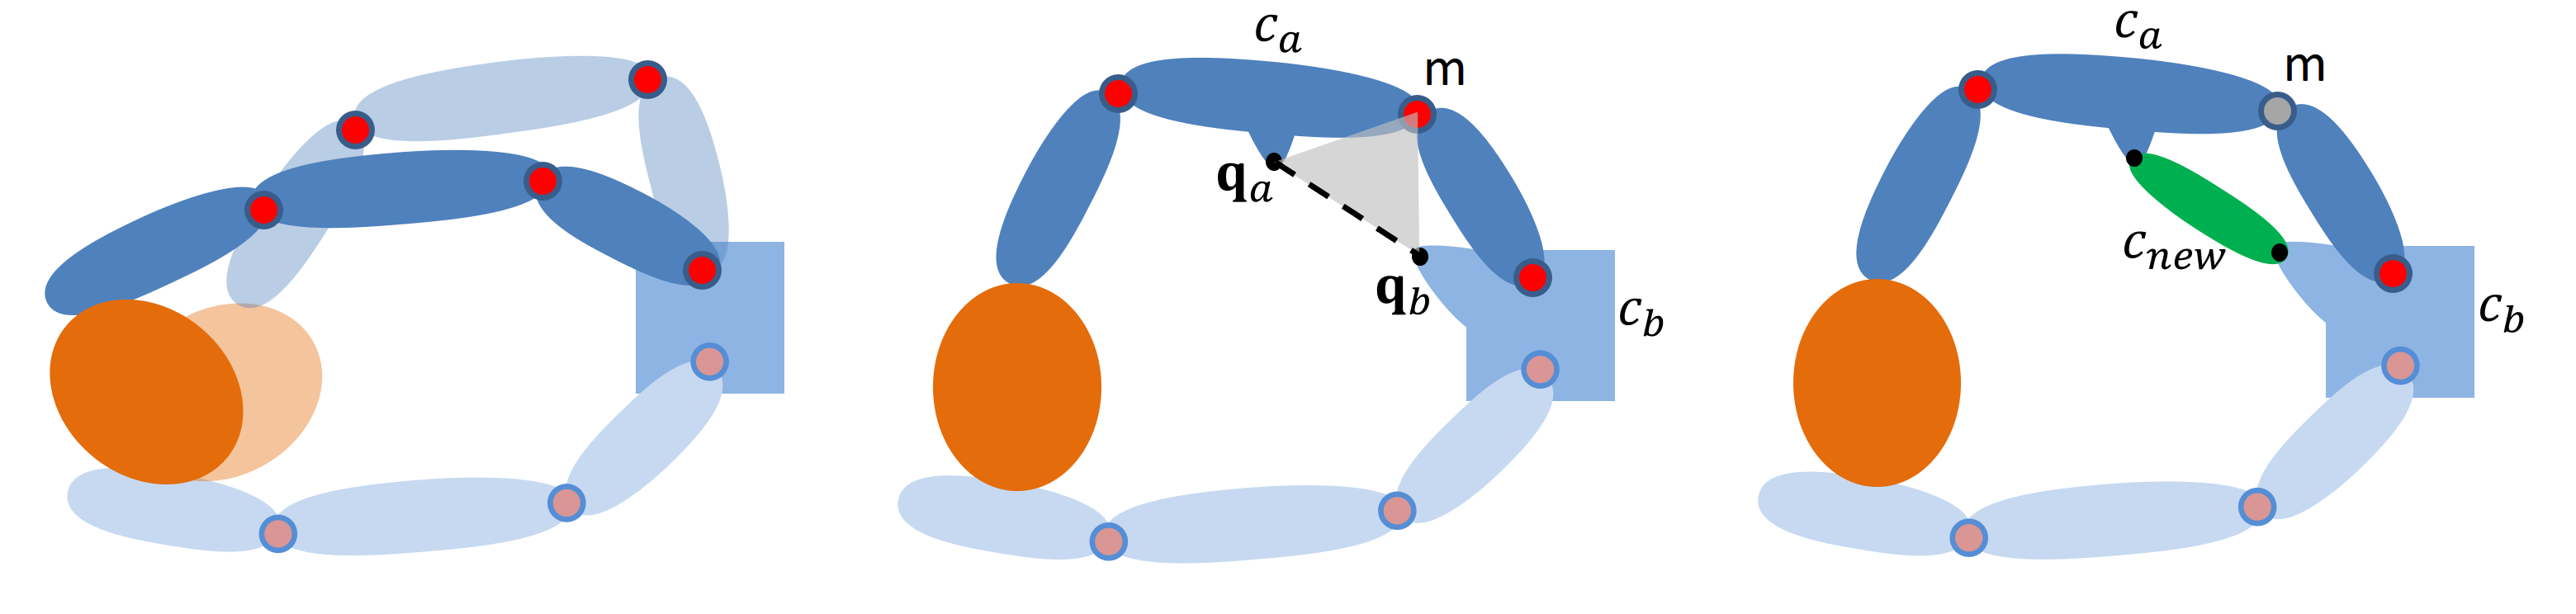
\includegraphics[width=6in]{./figs/handDesign.png}}
\end{center}
\vspace*{-0.2in}
\caption[]{(Left) A conceptual, fully actuated hand design performing a dexterous manipulation task. Active motors are highlighted in red. (Middle) Given two components $c_a$ and $c_b$, we seek a pair of points $\bq_a$ and $\bq_b$ such that the distance between them varies least throughout the motion. To avoid singularities, the area of the highlighted triangle must remain positive throughout the entire motion. (Right) The hand design is simplified by removing motor $m$ and introducing a new passive link $c_{new}$.}
\label{handMechanismDesign}
\end{figure}

\subsection{Top-down design}

While bottom-up approaches aim to create a hand design from scratch, we will also investigate top-down approaches. The strategy here will be to begin with a conceptual design of a highly actuated robot hand design. For example, if a dexterous manipulation task was described through motion capture data, then the initial design would be given by an actuated articulated structure that matches the kinematics of the performer's hand. The underlying assumption is that, with perfect state knowledge and optimal controllers, this robot hand would be able to perform the desired dexterous manipulation tasks. Through an iterative process, the mathematical models we will develop will be used to replace active degrees of freedom with appropriate passive mechanical structures such that a balance between adaptability and simplicity is achieved. 

Figure~\ref{handMechanismDesign} illustrates a conceptual, fully actuated robot hand consisting of rigid links connected to virtual actuators that control their motions. In principle, physical actuators could be used to directly replace their virtual counterparts when fabricating this robot hand. However, this would come at an increased cost, a more complex mechanical design setup, and it would require sophisticated control policies to coordinate all the actuators. As an alternative, we propose an automated design process that iteratively replaces virtual actuators with new rigid or compliant links that appropriately couple the motion of different parts of the hand mechanism. The attachment locations, length and material properties of the new mechanical components will be optimized such that changes to the functionality of the input hand design are minimized. 

The starting point for our investigations is a method recently developed by PI Coros and his colleagues. This method is used to design complex linkage structures that generate a desired motion trajectory~\cite{Thomaszewski14CDL}. The concept behind this method, which we will extend as part of our proposal, is based on a simple observation. Removing a motor and adding a new rigid link preserves the invariant that there are always as many constraints as degrees of freedom in the hand's mechanism: eliminating a motor removes one constraint, adding the (planar) link introduces three degrees of freedom, and two pin joints used to connect the new link to the existing structure result in four additional constraints. The motion of each mechanical component is thus either directly driven by a motor, or is mechanically coupled to that of other components.

To determine which motor should be replaced, and how to optimally insert a new mechanical component, we developed a mathematical model based on the following observation: if the distance $d$ between two points on a pair of existing components does not change as the hand performs a manipulation task, then these components can be connected through pin joints to a new rigid link of length $d$. Although the resulting mechanism would technically be over-constrained, the new link and its pin joints would be completely redundant. Removing a motor along the kinematic chain between the two components would resolve this redundancy while perfectly preserving the original motion. In general, there are no guarantees that such pairs of points always exist. Therefore, given two components, $c_a$ and $c_b$, we seek to find a pair of points $\bq_a$ and $\bq_b$ whose world-space distance varies least throughout the motion. The mean squared world-space distance between these two points is given by $l_{ab}=\frac{1}{n_s}\sum_i^{n_s}||\bq_a(t_i)-\bq_b(t_i)||^2$, where $n_s$ is a number of discrete time samples that span the entire motion, and the variance of this quantity is $ E_\mathrm{variance}=\frac{1}{n_s}\sum_i^{n_s}(||\bq_a(t_i)-\bq_b(t_i)||^2-l_{ab})^2$. When searching for the pair of points that minimize this variance term, it is critical that singular configurations are avoided at all times. As illustrated in Figure~\ref{handMechanismDesign}, when the selected motor ($m$) is removed, the new link ($c_{new}$) becomes responsible for driving the motion of component $c_a$ by direct coupling to component $c_b$. To ensure that the effective moment arm remains sufficiently large at all times, the area of the shaded triangle needs to always remain a safe distance away from zero. This can be accomplished through a log barrier term $E_\mathrm{area} = -\log\sum_i^{n_s}\text{area}\left(\bq_b(t_i),\bm(t_i),\bq_a(t_i)\right)^2$, where $\bm(t_i)$ denotes the world-space position for the motor $m$.

Given two components $c_a$ and $c_b$, which are selected in an outer loop, our mathematical model minimizes a weighted combination of the terms $E_\mathrm{variance}$ and $E_\mathrm{area}$. With gradients and hessians for these objectives readily available, a Newton-Raphson scheme efficiently solves the resulting optimization problem. Once points $\bq_a$ and $\bq_b$ are found, they define a candidate rigid link to be added to the hand mechanism. Our design system then individually removes each motor on the kinematic chain between $c_a$ and $c_b$ and further optimizes the motion of the resulting assembly using our recently developed method~\cite{Bacher2015}. Importantly, this optimization step not only adapts the kinematic parameters of the design, but also the actuator signals that control the motion of the hand mechanism. As a measure of the success of each potential replacement operation, we evaluate the difference in motion between the initial hand design and the optimized mechanism with fewer active degrees of freedom. If the resulting mechanisms deviate too much from the hand's initial motion, a new set of components will be selected and the process repeats. Otherwise, the replacement operation is finalized.

To improve the reliability of the designs generated with our mathematical models, we will develop additional optimization objectives based on the linear robustness analysis introduced by PI Pollard~\cite{Pollard:WAFR02,pollard2004closure,pollard20045}. Further, as described in the previous subsection, we will improve their adaptability by optimizing the compliance of the mechanical links introduced to replace active degrees of freedom. This significant extension will allow the simplified robot hands we design to not only duplicate motion trajectories, but also the contact forces required to manipulate objects.
% This initiative will build on recent methods developed by PI Coros to optimize volumetric~\cite{Skouras2013} and rod-based~\cite{Jesus2015} mechanical structures. Leveraging multi-material 3D Printing capabilities, our approach will therefore be able to reason not only in terms of the motion of the mechanical hand (and therefore the trajectory of the contact points) but also in terms of the contact forces applied to the objects being manipulated.

%compliance will be key
%duplicating motions will be the first step.
%prior work duplicated motions, here we will duplicate forces as well. 
%figure 3 left can go with figure 2
%figure 3 right can be a strip.
%add a quadruped robot pic in my strip
%upload facilities, follow up on budget justification

%In addition to optimizing the motion of the mechanical hand (which determines the contacts with the object being manipulated), our models will also need to reason about the forces that are being applied. Consequently, our models will modulate the compliance of the mechanical links that are introduced as active degrees of freedom are removed from the design. To achieve this goal, we will build on the work done by PI Coros in designing and optimizing volumetric~\cite{Skouras2013} and rod-based~\ref{Jesus2015} mechanical structures. Briefly, the relationship between displacements $\bu$ -- deformations away from a rigid configuration -- and forces $\bF$ is given by $\bF = K\bu$, where $K$ is a stiffness matrix that depends on material properties. 

%\subsection{Bottom-up Design}

%While top-down approaches rely on 

%

%We will be able to control the way in which torques generated by available motors get mapped to end effector forces.

%- task robustness
%- extensions to stops, forces, etc...

%Some random thoughts
%\begin{itemize}
%  \item Good simulations of the mechanisms that are being proposed are key and are very hard.   Can we get good material models?    Can we construct good models of uncertainties so that our simulation rollouts match our experiments?
%  \item Can we create a setup that allows lots of randomized tests for this purpose?    Making simulations match reality appears to be hot right now. 
%\end{itemize}

%\subsection{Cable-driven, continuously deforming structures}

%Talk about the option of starting with an elastically-deforming structure for each finger of the hand. We can either start with a large number of actuated virtual tendons, and figure out which to remove, or add them one by one, optimizing routing points.
